\section{Estrutura e Locomoção do robô} % (fold)
\label{sub:locomocao}
	
	O robô, de forma autônoma, deve percorrer todo o cômodo escolhido para limpá-lo para isso deve ser desenvolvido todo o sistema de locomoção dele, incluindo as rodas, motor, caixa de redução e todo o estudo dinâmico relacionado. Foram cogitadas duas soluções para a estrutura do robô e sua forma de locomoção, de forma que a segunda solução foi escolhida. A escolha da segunda solução se justifica com base nos requisitos do sistema de sensoriamento quanto a posição de sensores pela estrutura e devido ao maior erro propagado pela primeira solução na navegação inercial do sistema. 

	\subsection{Solução 1} % (fold)
	\label{sub:solução_1}
		
		O robô seria composto de uma chapa retangular de alumínio de 400mm x 300mm x 5mm, que servirá como base para a distribuição e união dos componentes do projeto. Essa base retangular poderá ser usinada para outra forma caso haja necessidade de diminuição do tamanho do robô. O material escolhido para a base foi o alumínio pela sua leveza, resistência e preço. Sua área  de superfície é capaz de abrigar todos os componentes do aspirador e ainda possui espaços para criar novas soluções ou até mesmo de componentes para a refrigeração dos subsistemas do robô.

		O sistema de tração dessa base será feito por uma esteira tipo lagarta, muito utilizada em tanques de guerra. Esse sistema é bastante robusto e aguentaria o peso de todo a estrutura sem problemas. Isso tiraria a necessidade de colocar um sistema de suspensão.

		A estrutura do aspirador e seus componentes:

		\begin{itemize}
			\item 2 motores com caixa de redução ligados a chapa de alumínio;
			\item Os eixos que ligaram as rodas a chapa de alumínio serão feitos com aço e serão usinados nas pontas para fazer roscas que irão fixar as rodas;
			\item 4 engrenagens grandes que serão utilizadas como rodas;
			\item 2 engrenagens menores que irão ser ligadas direto nos dois motores;
			\item Conectores múltiplos, do tipo que se usa em chuveiros para ligar os eixos na chapa de alumínio;
			\item Correntes de bicicleta que ligaram as engrenagens e farão o papel de esteira.
		\end{itemize}

		Entre esses dois sistemas foi escolhido o segundo pela sua construção ser mais robusta e suporta mais os esforços que será submetido o robô. Um grande problema do primeiro sistema é que a sustentação da estrutura se daria no próprio eixo do motor, que é de plastico, o que poderia causar a quebra do sistema, já no segundo sistema a sustentação é feita nos eixos, que são feitos de aço.
		
		\begin{figure}[H]
			\centering
			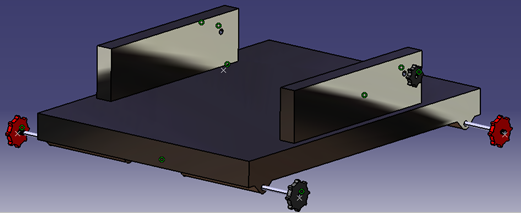
\includegraphics[scale=0.8]{figuras/rascunho_estrutura.png}
			\caption{Rascunho da estrutura - Solução 1}
			\label{img:rascunho1}
		\end{figure}


		\subsection{Solução 2} % (fold)
		\label{sub:solução_2}
			
			O robô aspirador terá forma circular. Esse formato foi escolhido para facilitar as manobras de curvas, aumentando a área que ele irá percorrer. Outra vantagem que esse formato fornece é a questão do controle autônomo dele, assim facilita a distribuição dos sensores e o próprio controle do movimento do robô, pois resulta em menos erros. A estrutura do robô deve ser tal para suportar as cargas dos equipamentos do interior do robô como os sensores, motores, coolers e o sistema de sucção sem que sofra deformações. Além dessas forças deve-se também ser resistente à fadiga, já que estará sujeito a cargas contínuas e repetidas, e a impactos contra objetos ou paredes.

            Em relação a movimentação do robô, três rodas estão sendo usadas para garantir o equilíbrio da estrutura, duas rodas com tração e uma livre, podendo ser adicionado uma segunda roda livre caso a disposição final dos componentes desequilibre o sistema.  A roda livre possui um giro de 360º facilitando o deslocamento, enquanto as outras duas rodas utilizam um kit motor-caixa de redução. A mudança de direção e giro do robô é realizada alternando a potência fornecida em cada roda ou invertendo o sentido de rotação, por exemplo para fazer com que ele gire para a esquerda, deve diminuir a potência da roda esquerda e manter a potência da roda direita. As figuras seguintes ilustram as rodas e motores utilizados.

			Um material que já é utilizado em muitas aplicações pois apresenta boa propriedades é o Alumínio. A tabela \ref{tab:rascunho1} mostra alguns valores das propriedades mecânicas do alumínio.


			\begin{table}[]
			\centering
			\caption{Propriedades mecânicas do alumínio. Adaptado de \href{http://www.shockmetais.com.br/especificacoes/aluminio/pmec}{Shockmetais}}
			\label{tab:rascunho1}
			\begin{tabular}{|c|c|}
			\hline
			Liga ABNT ASTM                                                                         & 1050                                             \\ \hline
			DIN                                                                                    & AI 99.5                                          \\ \hline
			Têmpera                                                                                & \begin{tabular}[c]{@{}c@{}}O\\ H14\end{tabular}  \\ \hline
			\begin{tabular}[c]{@{}c@{}}Limite de Resistência à Tração\\ Mpa(N/mm3)Min\end{tabular} & \begin{tabular}[c]{@{}c@{}}55\\ 95\end{tabular}  \\ \hline
			\begin{tabular}[c]{@{}c@{}}Limite de Resistência à Tração\\ Mpa(N/mm3)Max\end{tabular} & \begin{tabular}[c]{@{}c@{}}95\\ 130\end{tabular} \\ \hline
			\begin{tabular}[c]{@{}c@{}}Limite de Escoamento\\ Mpa(N/mm3)Min\end{tabular}           & \begin{tabular}[c]{@{}c@{}}15\\ 70\end{tabular}  \\ \hline
			\begin{tabular}[c]{@{}c@{}}Alongamento Mínimo\\ 50mm (\%)\end{tabular}                 & \begin{tabular}[c]{@{}c@{}}22\\ 3\end{tabular}   \\ \hline
			Dureza Brinnel (HB)                                                                    & \begin{tabular}[c]{@{}c@{}}20\\ 26\end{tabular}  \\ \hline
			\end{tabular}
			\end{table}

			Então será construída uma base circular de alumínio de 40 cm de diâmetro.

        	Com relação a movimentação do robô 3 rodas serão suficientes para garantir o equilíbrio. Duas rodas serão tracionadas uma livre.  A roda livre é do tipo esfera e as outras duas serão de um kit motor redução, que junto à roda está montado o motor com uma caixa de redução para aumentar o torque. A mudança de direção e giro do robô é realizada alternando a potência fornecida em cada roda ou invertendo o sentido de rotação, por exemplo para fazer com que ele gire para a esquerda, deve diminuir a potência da roda esquerda e manter a potência da roda direita. As figuras seguintes ilustram as rodas e motores utilizados.

        	\begin{figure}[H]
				\centering
				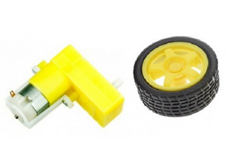
\includegraphics[scale=0.7]{figuras/motor_roda.png}
				\caption{Kit motor redução.}
				\label{img:kit_motor}
			\end{figure}

			\begin{figure}[H]
				\centering
				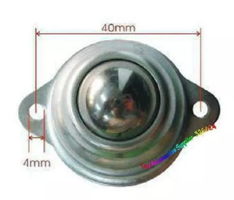
\includegraphics[scale=0.7]{figuras/esfera.png}
				\caption{Roda do tipo esfera.}
				\label{img:esfera}
			\end{figure}

			As especificações da roda e do motor são mostradas na tabela \ref{tab:motor_red}:

			\begin{table}[H]
				\centering
				\caption{Especificação motor de redução}
				\label{tab:motor_red}
				\begin{tabular}{|c|c|}
					\hline
					\multicolumn{2}{|c|}{\cellcolor[HTML]{C0C0C0}\textbf{Especificação Motor}} \\ \hline
					\textit{\textbf{Tamanho}}                            & 69x37x22,7mm        \\ \hline
					\textit{\textbf{Peso}}                               & 29g                 \\ \hline
					\textit{\textbf{Formato}}                            & 90 graus            \\ \hline
					\textit{\textbf{Tensão de operação}}                 & 3 a 6V              \\ \hline
					\textit{\textbf{Relação de transmissão}}             & 1:120               \\ \hline
					\textit{\textbf{Velocidade a 3V(sem carga)}}         & 100 rpm             \\ \hline
					\textit{\textbf{Corrente a 3V(sem carga)}}           & 60 mA               \\ \hline
					\textit{\textbf{Corrente a 3V(com carga)}}           & 260 mA              \\ \hline
					\textit{\textbf{Torque a 3V}}                        & 1.20 kgf-cm         \\ \hline
					\textit{\textbf{Velocidade a 6V(sem carga)}}         & 200 rpm             \\ \hline
					\textit{\textbf{Corrente a 6V(sem carga)}}           & 71 mA               \\ \hline
					\textit{\textbf{Corrente a 6V(com carga)}}           & 470 mA              \\ \hline
					\textit{\textbf{Torque a 6V}}                        & 1.92 kgf-cm         \\ \hline
					\textit{\textbf{Diâmetro externo do eixo}}           & 5,4 mm "I"          \\ \hline
				\end{tabular}
			\end{table}

			\begin{figure}[H]
				\centering
				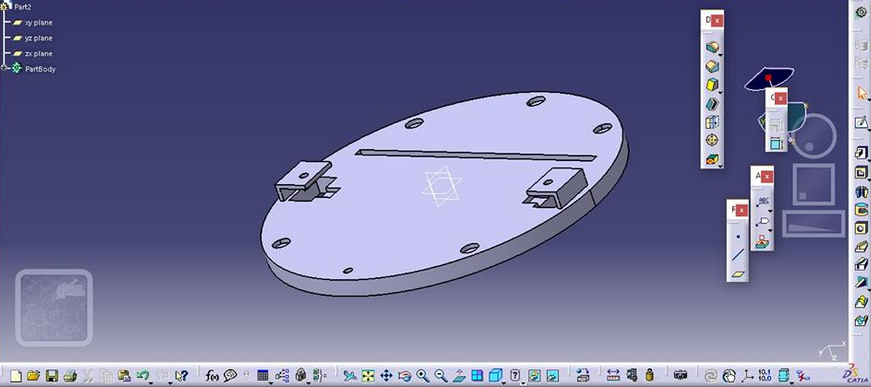
\includegraphics[scale=0.5]{figuras/estrutura_circular.png}
				\caption{Estrutura circular de integração dos subsistemas.}
				\label{img:estrutura_circular}
			\end{figure}

			\begin{table}[H]
				\centering
				\caption{Especificações roda tracionada}
				\label{tab:especificacoes_roda}
				\begin{tabular}{|c|c|}
					\hline
					\multicolumn{2}{|c|}{\cellcolor[HTML]{C0C0C0}\textbf{Especificação da Roda}}                 \\ \hline
					\textit{\textbf{Material}}                             & Roda plástica com pneu de borracha. \\ \hline
					\textit{\textbf{Diâmetro externo}}                     & 65 mm                               \\ \hline
					\textit{\textbf{Largura pneu}}                         & 26 mm                               \\ \hline
					\textit{\textbf{Diâmetro interno para engate do eixo}} & 5,4 mm "I"                          \\ \hline
				\end{tabular}
			\end{table}

			A parte superior da estrutura, ou seja, a tampa, será fabricada em PVC ou em acrílico. A escolha de um material plástico deve-se a facilidade de manuseio, facilitando molda-lo à forma desejada. Deixa a estrutura mais leve, fazendo com que o motor realize menos trabalho, e pode suportar valores altos de cargas, resistindo a impactos. O material acrílico (METACRILATO DE METILA) possui (densidade relativa de 1.19 g/cm3), resistente a água e boa resistência segundo a Tabela \ref{acrilico}:
						
			\begin{table}[H]
			\centering
			\caption[Valores de propriedades mecânicas do Acrílico]{Valores de propriedades mecânicas do Acrílico. Adaptado de \href{http://www.indac.org.br/arquivos/acrilico\_indac.pdf}{Indac}.}
			\label{acrilico}
			\begin{tabular}{lll|l|l|}
			\cline{4-5}
			\textbf{}                                                    & \textbf{}                                      & \textbf{}        & \textbf{Valores}     & \textbf{Valores}    \\ \hline
			\multicolumn{1}{|l|}{\textbf{Mecânicas}}                     & \multicolumn{1}{l|}{\textbf{Método de Ensaio}} & \textbf{Unidade} & \textbf{Chapas Cast} & \textbf{Extrusadas} \\ \hline
			\multicolumn{1}{|l|}{Resistência à Tração}                   & \multicolumn{1}{l|}{ISO 527}                   & MPa              & min 70               & min 60              \\ \hline
			\multicolumn{1}{|l|}{Resistência à Flexão}                   & \multicolumn{1}{l|}{ISO 178}                   & MPa              & 110                  & 110 a 115           \\ \hline
			\multicolumn{1}{|l|}{\textit{Resistência ao impacto Charpy}} & \multicolumn{1}{l|}{ISO 179/1fU}               & KJ/m2            & min 13               & min 8               \\ \hline
			\multicolumn{1}{|l|}{Dureza Rockwell}                        & \multicolumn{1}{l|}{ISO 2039-2}                & Escala M         & 100                  & 90 a 95             \\ \hline
			\end{tabular}
			\end{table}

			Na tabela \ref{tab:pvc} são apresentados os valores referentes ao PVC.

			\begin{table}[H]
				\centering
				\caption{Valores das propriedades mecânicas do PVC.	}
				\label{tab:pvc}
				\begin{tabular}{|c|c|c|c|}
					\hline
					\textit{\textbf{Materiais}} & \textit{\textbf{\begin{tabular}[c]{@{}c@{}}Resistência a tração\\ (N/mm\textsuperscript{2})\end{tabular}}} & \textit{\textbf{\begin{tabular}[c]{@{}c@{}}Módulo de elasticidade\\ (kN/mm\textsuperscript{2})\end{tabular}}} & \textit{\textbf{\begin{tabular}[c]{@{}c@{}}Densidade\\ (kg/m\textsuperscript{3})\end{tabular}}} \\ \hline
					PVC                         & 55                                                                                       & 3.5                                                                                         & 1400                                                                          \\ \hline
				\end{tabular}
			\end{table}

			O PVC e o acrílico apresentam um modulo de elasticidade e resistência a tração compatíveis com as necessidades estruturais do projeto. O PVC possui um fácil manuseio, um preço compatível e é fácil de encontrar no mercado. O acrílico exige cuidados para a realização de usinagem, devido a alta fragilidade.
	% subsection solução_1 (end)
% section alimentação (end)
